
\section{Requirements specification for Main Application Module}\label{Requirements specifications for Main Application Module}
\subsection{General Definition}\label{GeneralDefinition main}
Main Application Module (MAM) is an application, which responsible for management N2Sky system. It embeds:
\begin{itemize}
\item Model Repository 
\item Neural Network Repository 
\item N2Sky Main Dashboard.
\end{itemize}

MAM is a core component of the N2Sky platform. From this component, users can feel the power of the N2Sky system and try out the whole functionality of it. The MAM, as well as other N2Sky components, is possible to use on any device because it supports responsive design. 

\subsection{Affected users}\label{Affected users MAM}
The MAM has one User Interface but users can use it diverse. Only users, which the main function is within MAM can operate this module on their own purpose. Following types of users have this kind of the main function:

\begin{itemize}
\item \emph{Arbitrary User.} The main function of the arbitrary user is to learn about neural networks or try out his knowledge in this field. The typical use case is when the user logs in from the mobile device like smartphone all tablet and search something in repositories. This user copy existing neural networks or trained models into own project and perform some operations on it.  A detailed description is in \autoref{User Roles}. 
\item \emph{Neural Network Engineer User.} This kind of user normally uses Desktop version of N2Sky, but he can also use the mobile version because all functionalities are also available there. The user creates own neural network from existing paradigm, but he also can act as an Arbitrary User.  A detailed description is in \autoref{User Roles}. 
\item \emph{Contributor User.} The Contributor uses N2Sky MAM component mostly for an easier way to check his own neural network paradigm. Since this user can fully use N2Sky open API, UI for him is just for the quick check. The UI is available also in the mobile version, that is why Contributor can observe his neural networks behavior directly from the mobile device in any place. A detailed description is in \autoref{User Roles}. 
\item \emph{System Administrator.} His main function is on AM module, but since he is also the administrator of the N2Sky MAM he can see all processes of other users. This user can shadow any other user in order to see what is happening in particular user dashboard.  A detailed description is in \autoref{User Roles}. 
\end{itemize}

\subsection{N2Sky Dashboard}\label{N2Sky Dashboard}
The N2Sky dashboard is the central component of the MAM module. The dashboard gives brief information about available tools, user's projects and user's neural networks. Every dashboard is unique for every user, namely the content is always differ. As it is displayed in figure \ref{fig:n2skymaindashboard}, the dashboard gives full overview of the components from one page.

\begin{figure}[htbp]
\begin{center}
  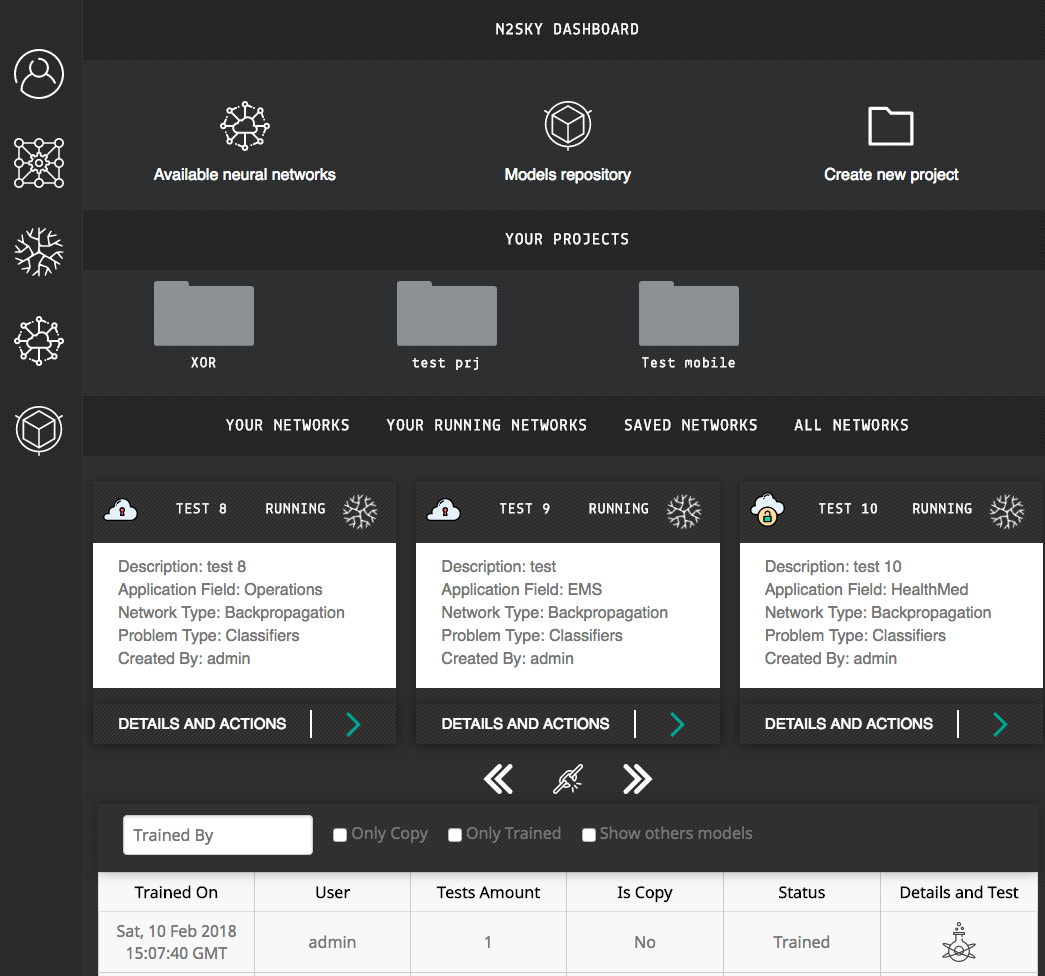
\includegraphics[width=\linewidth]{components/5/img/n2sky_main_dashboard.png}
  \caption{N2Sky User Dashboard}
  \label{fig:n2skymaindashboard}
\end{center}
\end{figure}

The N2Sky dashboard contains following components:
\begin{itemize}
\item Available tools
\item The user projects
\item The user neural networks 
\item The user trained models
\end{itemize}

The dashboard is available under following URL path:
 \begin{lstlisting}
	<host>/cloud
\end{lstlisting}

\subsubsection{Available tools}

\begin{figure}[htbp]
\begin{center}
  
\includegraphics[scale=0.5]{components/5/img/n2sky_tools.png}
  \caption{N2Sky Main Module. Available user tools}
  \label{fig:n2sky_tools}
\end{center}
\end{figure}

In figure \ref{fig:n2sky_tools} the available tools component is displayed in a horizontal layout. Every item has an SVG icon and caption under it. The tools contain following functionalities: 
\begin{itemize}
\item \emph{Available neural network.} Reference to the available repositories view.  
\item \emph{Model repository.} Reference to the model repository view.
\item \emph{Create new project.} On click of this time the popup window will me initialised as it displayed in figure \ref{fig:popupcreatenewproject}.


\begin{figure}[htbp]
\begin{center}
  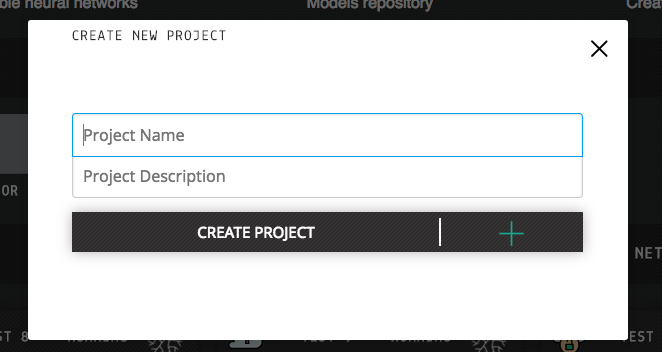
\includegraphics[scale=0.5]{components/5/img/popupcreatenewproject.png}
  \caption{N2Sky Main Module. Create New Project Popup}
  \label{fig:popupcreatenewproject}
\end{center}
\end{figure}


The following popup modal window contains components:
\begin{itemize}
\item \emph{Project Name} field, which represents a short title of the project.
\item \emph{Project Description} field with a short description of the project, which will be user for semantic search.  
\item \emph{Create Project} button, which created a project with filled up form.
\end{itemize}

After creating the project it will be automatically appear in the dashboard. 

\end{itemize}

\subsubsection{User projects}

User projects is a grid with projects. Every project is represented as a folder with a caption under it as it displayed in figure \ref{fig:n2sky_dashboard_projects}. On click the user will be redirected to the particular project. 

\begin{figure}[htbp]
\begin{center}
  
\includegraphics[scale=0.5]{components/5/img/n2sky_dashboard_projects.png}
  \caption{N2Sky Main Module. User projects grid}
  \label{fig:n2sky_dashboard_projects}
\end{center}
\end{figure}

 \subsubsection{The user neural networks and models overview}
 
 The component is displaying the neural networks of the user, which either created from paradigm or own contributed neural networks. The component contains following subcomponents:
 \begin{itemize}
\item \emph{Neural networks filtering bar.}
The filtering bar is a navigation as well as neural networks filtering subcomponent as it shown in figure \ref{fig:n2sky_filtering_bar}. The subcomponent allows user to filter through neural networks depending on permissions. 

\begin{figure}[htbp]
\begin{center}
  
\includegraphics[scale=0.5]{components/5/img/n2sky_filtering_bar.png}
  \caption{N2Sky Main Module. Neural networks filtering bar.}
  \label{fig:n2sky_filtering_bar}
\end{center}
\end{figure}

The following filters are available: 
\begin{itemize}
\item \emph{Your networks.} The filter shows the running and not running neural networks of the logged in user. 
\item \emph{Your running networks.} The representation only of the user's running neural networks.
\item \emph{Saved networks.} Only saved neural networks of the users. The list will show the saved neural networks across all projects of the user.
\item \emph{All Networks}. List of the all networks on the N2Sky. This filter is available only for system administrator.
\end{itemize}
\item{The neural networks grid.} The grid, which contains custom UI components that represents particular neural network. Every grid item contains following information:
\begin{itemize}
\item The title of the neural network
\item The status tither running or not running. If the instance is running the N2Sky icon will spin, if not it will be grey without movements. 
\item The short description of the neural network
\item Application field
\item Network type
\item Problem type
\item Created by user
\item Details and actions button, which redirect the user to the page with detailed information of the neural network. 
\end{itemize}

\item{Navigation bar.} The bar under neural networks which contains the navigation buttons and "Chained/Unchained" mode.
\begin{itemize}
\item \emph{Unchained mode} is a mode where all trained model of displayed neural networks will be shown.
\item \emph{Chained mode} is a mode where only the trained models of chosen neural network will be shown. In chained mode the user hast to click on particular neural network to see the trained models. 
\end{itemize}

\item{Trained models table.} The table with trained models, which contained also filtering and searching bar.
The filtering and searching bar allows to perform semantic search across trained models and contains following filters:
\begin{itemize}
\item Trained by field available only for contributor user and system administrator.
\item Only Copy checkbox
\item Only Trained checkbox means show only the trained models where the training is finished.
\item Show others modes checkbox will display the trained models from other users. The checkbox available only to system administrator.
\end{itemize}

The table itself contains short information about the trained models. On click the user will be redirected to detailed overview of the trained model.


\end{itemize}



\subsection{Neural Networks Repository}\label{Neural Networks Repository}
\subsection{Models Repository}\label{Models Repository}
